\documentclass[a4paper, 12pt]{article}
\usepackage{graphicx}
\usepackage{amsmath}
\usepackage[utf8]{inputenc}
\usepackage[T1]{fontenc}
\begin{document}

\title{Lorem ipsum dolor sit.}
\author{Konrad Kreczko}
\date{\today}

\tableofcontents
\newpage



\maketitle
\newpage
\begin{abstract}
Lorem ipsum dolor sit amet, consectetur adipiscing elit. Pellentesque porttitor ante convallis ligula vestibulum blandit. Aliquam erat volutpat. Integer quis malesuada erat. Nunc placerat, elit vitae rutrum mollis, enim sem cursus augue, quis faucibus ante orci gravida libero. Aenean commodo iaculis ante. Nullam sit amet magna interdum, elementum tortor vitae, scelerisque augue. Nunc erat ipsum, dapibus quis varius quis, aliquet tincidunt sapien. Nam blandit orci ut mauris tristique, sit amet accumsan mi accumsan. Etiam fringilla nunc ut ornare venenatis. Praesent eu finibus felis \cite{5}.
\end{abstract}
\newpage
\section{Lorem ipsum dolor.}
\subsection{Quisque feugiat}
Lorem ipsum dolor sit amet, consectetur adipiscing elit. Proin id nisi sagittis tortor lacinia egestas eu eget orci. Cras id nisi lectus. \textbf{Pellentesque} egestas lorem scelerisque nisi varius suscipit. Cras convallis tortor ac finibus vulputate. Nam consequat nisi mattis eros convallis, ut faucibus elit tincidunt. Praesent varius et enim ac tincidunt. In scelerisque, quam vitae posuere fermentum, turpis est tempus risus, at malesuada ligula enim a ligula. Morbi libero turpis, condimentum pretium magna egestas, gravida fringilla magna. Nullam finibus ligula elit, sit amet lacinia quam dapibus nec. Suspendisse ultricies blandit elementum. In hac \textbf{habitasse} platea dictumst. Vestibulum vel odio tempus, rutrum justo a, dignissim turpis. Mauris cursus dolor vel elit tincidunt, nec interdum arcu sodales. Sed quis purus quis massa ullamcorper volutpat eu eget arcu.

Etiam sagittis nisl risus, sed egestas \cite{6} ligula gravida quis. Duis vel mauris libero. Phasellus metus purus, pretium non metus at, bibendum blandit lorem. Sed imperdiet nunc libero, at scelerisque ante tristique sed. Aliquam vel nisi bibendum, rutrum odio ut, hendrerit justo. Nulla pellentesque justo vitae leo laoreet, sit amet lobortis erat elementum. Praesent dapibus \underline{commodo} facilisis. Nulla vel tellus non justo aliquam tincidunt eget sit amet neque. Donec congue nec purus faucibus fermentum. Sed rhoncus placerat metus id iaculis. Duis tincidunt semper consectetur.

\begin{equation}
x = \frac{-b \pm \sqrt{b^2 - 4ac}}{2a}
\end{equation}

Praesent nec neque at elit vehicula egestas vitae a mauris. Mauris sollicitudin velit urna, bibendum eleifend purus vestibulum id. \underline{Vivamus consectetur} a sem a molestie. Phasellus in rhoncus turpis. Vestibulum ante ipsum primis in faucibus orci luctus et ultrices posuere cubilia curae; Phasellus accumsan sem nisl, in convallis risus porttitor luctus. Nullam malesuada lectus sit amet mi aliquam convallis.
\begin{equation}
A = \begin{bmatrix}
a_{11} & a_{12} & \dots & a_{1n} \\
a_{21} & a_{22} & \dots & a_{2n} \\
\vdots & \vdots & \ddots & \vdots \\
a_{m1} & a_{m2} & \dots & a_{mn} \\
\end{bmatrix}
\end{equation}

\subsection{Lorem ipsum dolor sit amet}

Lorem ipsum dolor sit amet, consectetur adipiscing elit. Proin id nisi sagittis tortor lacinia egestas eu eget orci. Cras id nisi lectus. Pellentesque egestas lorem scelerisque nisi varius suscipit. Cras convallis tortor ac finibus vulputate. Nam consequat nisi mattis \cite{4} eros convallis, ut faucibus elit tincidunt. Praesent varius et enim ac tincidunt. In scelerisque, quam vitae posuere fermentum, turpis est tempus risus, at malesuada ligula enim a ligula. Morbi libero turpis, condimentum pretium magna egestas, gravida fringilla magna. Nullam finibus ligula elit, sit amet lacinia quam dapibus nec. Suspendisse ultricies blandit elementum. In hac habitasse platea dictumst. Vestibulum vel odio tempus, rutrum justo a, dignissim turpis. Mauris cursus dolor vel elit tincidunt, nec interdum arcu sodales. Sed quis purus quis massa ullamcorper volutpat eu eget arcu.
\begin{equation}
\sum_{n=1}^\infty \frac{1}{n^2} = \frac{\pi^2}{6}
\end{equation}

\section{Etiam sagittis nisl risus}
\subsection{Phasellus metus purus}
Etiam sagittis nisl risus, sed egestas ligula gravida quis. Duis vel mauris libero. Phasellus metus purus, pretium non metus at, bibendum blandit lorem. Sed imperdiet nunc libero, at scelerisque ante tristique sed. Aliquam vel nisi bibendum, rutrum odio ut, hendrerit justo. Nulla pellentesque justo vitae leo laoreet, sit amet lobortis erat elementum. Praesent dapibus commodo facilisis. Nulla vel tellus non justo aliquam tincidunt eget sit amet neque. Donec congue nec purus faucibus fermentum. Sed rhoncus placerat metus id iaculis. Duis tincidunt semper consectetur.

Praesent nec neque at elit vehicula egestas vitae a mauris. \cite{3} Mauris sollicitudin velit urna, bibendum eleifend purus vestibulum id. Vivamus consectetur a sem a molestie. Phasellus in rhoncus turpis. Vestibulum ante ipsum primis in faucibus orci luctus et ultrices posuere cubilia curae; Phasellus accumsan sem nisl, in convallis risus porttitor luctus. Nullam malesuada lectus sit amet mi aliquam convallis.

\subsection{Etiam et enim ut purus posuere euismod.}
Maecenas iaculis lectus lorem, in placerat sapien iaculis vitae. Etiam vehicula lorem non urna dignissim, eget semper ante molestie. Sed sit amet sollicitudin lacus. Nulla rutrum magna in enim lacinia dapibus. Duis lacinia mi ipsum, in consectetur arcu maximus sed. Morbi cursus ultrices magna. Donec justo tellus, posuere a tempus sed, pellentesque faucibus dui. Curabitur mattis turpis eu ultrices cursus. Aliquam mattis metus augue, sed sodales purus condimentum rhoncus. Cras tincidunt vestibulum dui vitae vehicula. Suspendisse ultricies nibh sit amet mauris fermentum volutpat. Quisque pharetra consequat nunc semper scelerisque. Ut accumsan aliquet dui ac efficitur.

\begin{figure}[htp]
\centering
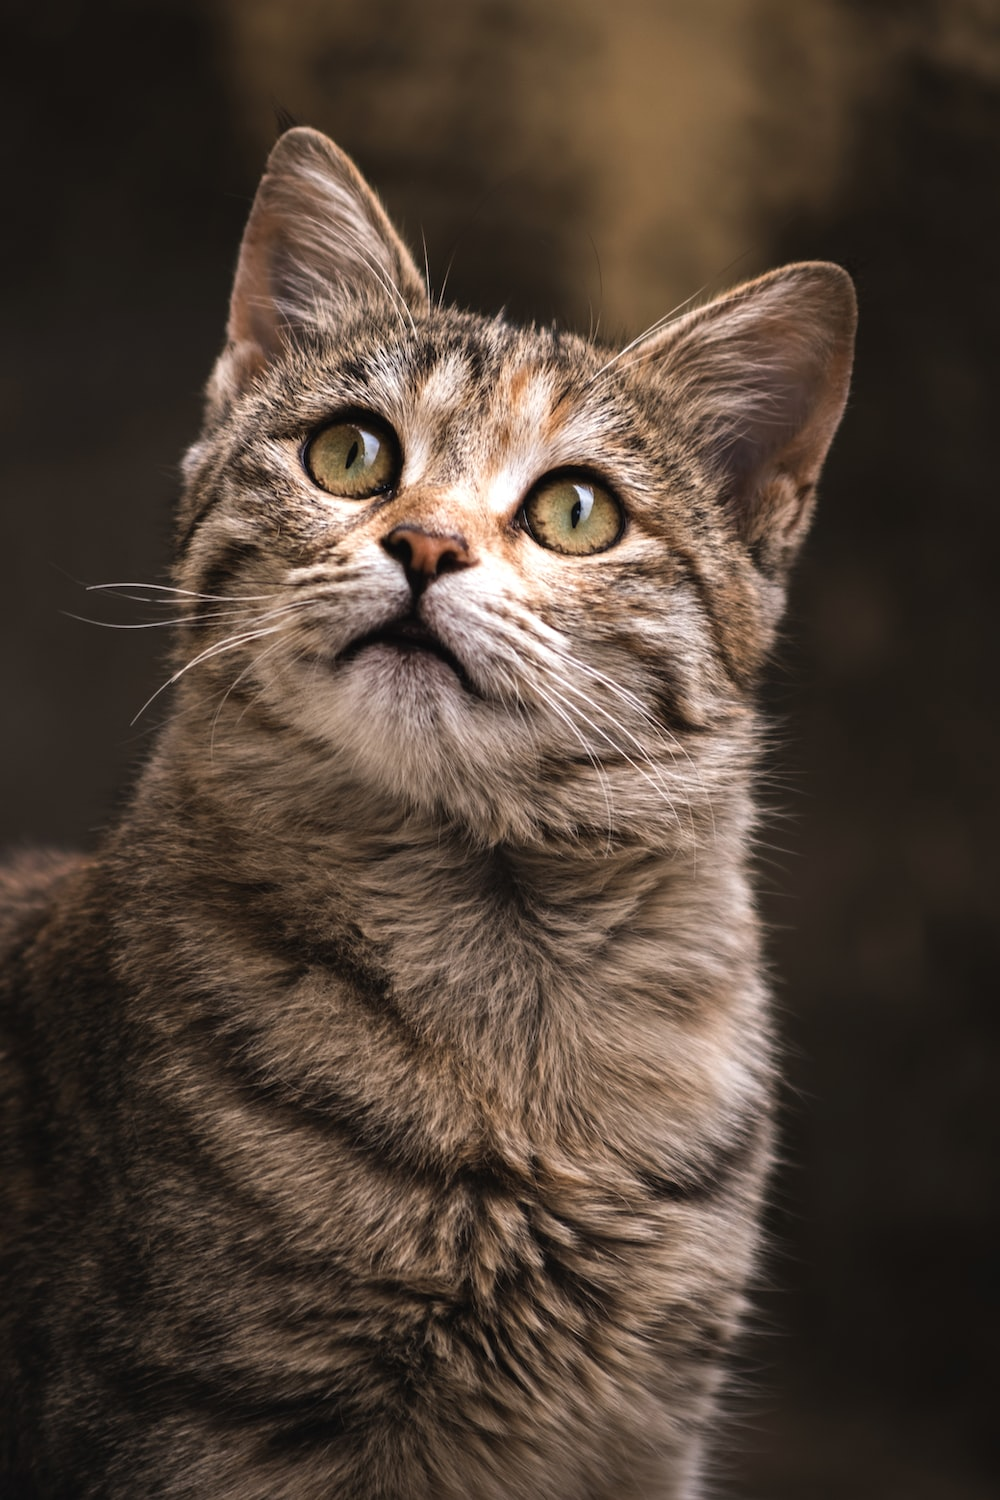
\includegraphics[width=0.3\textwidth]{image1.png}
\caption{Poważny \textbf{kiciuś} Więcej o kotach w świetnej książce \cite{1}.}
\label{obraz1}
\end{figure}

Maecenas cursus libero in lacus fringilla placerat. Vivamus et scelerisque ipsum, id mattis ipsum. Donec a luctus ligula, vitae tincidunt elit. Phasellus eros ipsum, vehicula ac pretium id, congue eget turpis. Fusce quis lacinia lacus, sit amet tristique eros. Donec faucibus lectus purus, posuere convallis metus eleifend eget. Proin blandit ex ac ultricies tincidunt. Proin purus diam, tincidunt nec magna eget, blandit placerat velit.

\subsection{Praesent nibh mauris}
Curabitur non rutrum massa, sit amet feugiat massa. Cras tristique lacinia rutrum. Quisque iaculis dictum ligula, vel facilisis nibh ultricies ac. Cras eleifend augue et volutpat blandit. In mollis posuere nunc, non tincidunt lacus consequat eu. Etiam hendrerit urna nibh, quis ornare ex imperdiet eu. Aliquam vitae congue metus. Sed ultrices ante id justo varius ornare. Donec posuere mi felis, sed gravida lorem posuere a. Proin consequat finibus varius. Sed aliquam ipsum dui, id facilisis risus rutrum vel. Fusce laoreet laoreet diam, eu iaculis lacus rhoncus eu. Etiam elementum porttitor mauris, nec faucibus felis condimentum in. Curabitur id ullamcorper tortor. Sed elementum elit \cite{2} id eros posuere, ac ornare dolor auctor. Praesent dignissim eget ligula nec tincidunt.

\begin{figure}[htp]
\centering

\includegraphics[width=0.3\textwidth]{image.png}
\caption{Słodki \textbf{kot} Więcej o kotach w świetnej książce \cite{1}.}
\label{obraz2}
\end{figure}

\centering
\begin{tabular}{|l|l|l|}
\hline
Nullam & Phasellus & Mauris  \\ \hline
243 & 1101 & 110002\\ \hline
230 & 250 & 2455\ \\ \hline
1112 & 1123 & 1234\ \\ \hline
\end{tabular}

\newline
\caption{Tabela z \textbf{nagłowkami} w postaci losowych słów z tekstu, a pod nimi przypadkowe liczby.}


\begin{figure}[htp]
\textbf{Podsumowując}, kot szary \ref{obraz1} jest poważny, a kot rudy \ref{obraz2} słodki.
\end{figure}
\newpage
\bibliographystyle{unsrt}
\bibliography{data}

\end{document}
